\documentclass[11pt]{paper}
\usepackage{palatino}
\usepackage{amsfonts,amsmath,amssymb}
% \usepackage{graphicx}

\usepackage{listings}
\usepackage{textcomp}
\usepackage{color}

\definecolor{dkgreen}{rgb}{0,0.6,0}
\definecolor{gray}{rgb}{0.5,0.5,0.5}
\definecolor{mauve}{rgb}{0.58,0,0.82}

\lstset{frame=tb,
  language=R,
  aboveskip=3mm,
  belowskip=3mm,
  showstringspaces=false,
  columns=flexible,
  basicstyle={\small\ttfamily},
  numbers=none,
  numberstyle=\tiny\color{gray},
  keywordstyle=\color{blue},
  commentstyle=\color{dkgreen},
  stringstyle=\color{mauve},
  breaklines=true,
  breakatwhitespace=true,
  tabsize=3
}



\ifx\pdftexversion\undefined
    \usepackage[dvips]{graphicx}
\else
    \usepackage[pdftex]{graphicx}
    \usepackage{epstopdf}
    \epstopdfsetup{suffix=}
\fi

\usepackage{subfig}


% This allows pdflatex to print the curly quotes in the
% significance codes in the output of the GAM.
\UseRawInputEncoding

\begin{document}
%%%%%%%%%%%%%%%%%%%%%%%%%%%%%%%%%%%%%%%%
% Problem Set 7
%%%%%%%%%%%%%%%%%%%%%%%%%%%%%%%%%%%%%%%%

\pagestyle{empty}
{\noindent\bf Spring 2021 \hfill Ali Berra}
\vskip 16pt
\centerline{\bf University of Central Florida}
\centerline{\bf College of Business}
\vskip 16pt
\centerline{\bf QMB 6911}
\centerline{\bf Capstone Project in Business Analytics}
\vskip 10pt
\centerline{\bf Final Project: Car Data}
\vskip 32pt
\noindent
% 

%%%%%%%%%%%%%%%%%%%%%%%%%%%%%%%%%%%%%%%%
\section{Introduction}

From the article "The Market for "Lemons": Quality Uncertainty and the Market Mechanism" talks about when purchasing a used car, the buyer faces an information problem, namely, they do not know if the car will be a good or a lemon.Unlike other goods, defective cars are difficult to identify due to the complex nature of the car-manufacturing process. In addition, the seller has an incentive to hide information about the car (number of repairs, manufacturing defects, etc.) in order to obtain the highest price possible.This leads to a risk-averse buyer where they underpay for used cars due to the uncertainty involved with the purchase.This summarizes to a infomational asymmetry,where some parties have information that others do not,causing the market to collapse and worhtless cars to trade around zero.
Market mechanisms such as brand naming and entrepreneurs taking advantage of profit oppurtunites is discussed by Akerlof. But the author goes beyond and extrapolates the used-car market example to other goods or services.He applies the Lemon Model to the health insurance industry, this is a great example to show rise to inefficiencies due to adverse selection and information asymmetries.He asks a question " why doesn't the price rise to match the risk?"In other words, to avoid adverse selection, health insurance companies are especially cautious when it comes to insuring older people or people that are more prone to get sick (to use the author’s terminology, lemons). According to Akerlof, this is an argument in favor of government intervention in health care.Akerlof’s paper is of the utmost importance for pointing out that information asymmetries could potentially cause a suboptimal allocation of resources. Yet the main example he employs to make his case about the market for used cars, does not show substantial market-coordination problems that can’t be overcome through other market mechanisms. In addition, adverse selection does not seem to apply to the health insurance industry, at least not in an important and substantial manner.He also uses minorities in the job market and credit markets in underdeveloped countries to show how "dishonesty" tend to drive honest dealings out of the market.Thats why licensing and brand names are a more secure and dependable purchase compared to trusting a seller to get a "lemon".

\vskip 32pt







Important features of pre-owned vehicle market.  
\vskip 12pt
The most important features that people look for when buying a used car can be summarized in four sections: overall conditions, accident history, service history, make and milage. 
\vskip 12pt
Overall condition can be looked at the overall condition of the vehicle like wear and tear, the exterior and interior look and the milage. The overall can be very useful to determine the price of used car, and people with small budget will look for a car that is older and with a medium overall condition if we can say. 
\vskip 12pt
Accident history, which can be a deal breaker for a lot of customers before making the decision on buying a used car or not. Because damaged car will be a lost for the buyer and can cause other expenses. 
\vskip 12pt
Service history, also like accident history is very important to buyers. A missing the regular service suggested by the manufacturer will cause damage to the vehicle and therefore more expenses for the buyers.  A good service will provide the buyers with secure decision. 
\vskip 12pt
Make and mileage, can be a good indicator of the price of used car because Japanese vehicle like Toyota or Nissan are known to last longer than European cars for example. 




\vskip 20pt



Table of features of used cars that can be used to determine their price







\begin{table}[ht]



\centering



\begin{tabular}{rlrrrrr}



\hline



Price&Overall condition&Accident History&Service History& Make and Mileage\\


\hline


Price 1 &good&1&poor&Honda 120k\\


Price 2 &good&1&good&Toyota 50k \\


Price 3 &good&1&poor&Honda 120k \\


Price 4 &medium&1&good&Mazda 120k \\


\hline

\end{tabular}

\caption{Prices of used cars by features}

\label{tab:summary}

\end{table}


\vskip 12pt

Lancaster and hedonic price theory can be used in theorical structure like used cars.
\vskip 12pt
In Lancaster model consumer look at purchased good as a bundle of characteristics, like in our example used car have multiple features that can be decisive for buyers. Like for example one buyer with high budget is looking for German car with low milage and very good condition of the interior and exterior. Another buyer with lower budget can be looking for different characteristics, like Japanese maker and reliable car for example. 
\vskip 12pt
Concerning Hedonic Pricing Method, it will be useful to determine values of used cars and drive conclusions. Because it will allow to determine the value of a vehicle by accounting the various factors that influence the price. 

Sample selection 
\vskip 12pt
Sample selection can be influential in the final model because of bias and that can be explained by choosing a non-random data. Which can reflect a different estimator of the population, and miss-representation of the population

\clearpage
%%%%%%%%%%%%%%%%%%%%%%%%%%%%%%%%%%%%%%%%
\section{Data Description}

This analysis follows the script \texttt{Car\_Reg\_Model.R} to produce a more accurate model for used trucks cost with the data from \texttt{UsedTrucks.dat} in the \texttt{Data} folder. 
The dataset includes the following variables.
\begin{table}[h!]
\begin{tabular}{l l l}

$type_i$ & = & sale type \\

$pauc$ & = & price when sold at auction \\
$ pret$ & = &price when sold retail \\ 
$mileage$ & = & odometer \\ %, $0$ otherwise \\
$make$ & = &make of vehicule \\
$year$ & = &model year of vehicle \\ 
$damage$ & = & an index of damage to vehicle, 1 little damage, 10 a lot\\
$dealer$ & = & dealer id \\ 
$ror$& = &rate-of-return\\
$cost$& = &net amount given to trade in\\


\end{tabular}
\end{table}
%
\clearpage
%%%%%%%%%%%%%%%%%%%%%%%%%%%%%%%%%%%%%%%%
\section{Analysis of the Dependent Variable}



Figure  \ref{fig:ecdf_ror} is 
a plot of the empirical cumulative distribution function (CDF) of rate of return. 


\begin{figure}[h!]
  \centering
  
\includegraphics[scale = 0.5, keepaspectratio=true]{../Figures/ecdf_ror}
  \caption{Empirical Distribution Function of rate of return} \label{fig:ecdf_ror}
\end{figure}

\subsection{Relative Histogram of ROR}

Figure \ref{fig:hist_ror} is 
a histogram of ROR. 

\begin{figure}[h!]
  \centering
  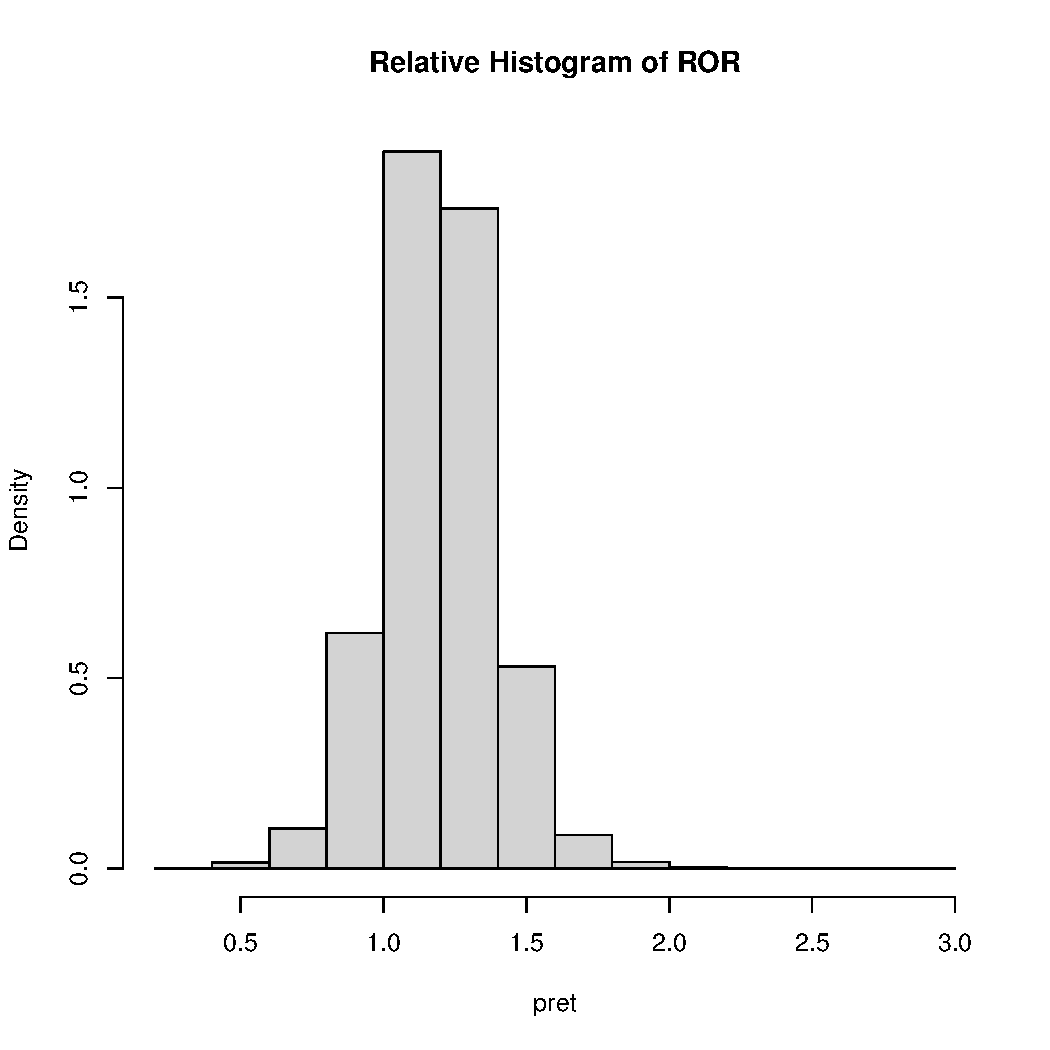
\includegraphics[scale = 0.5, keepaspectratio=true]{../Figures/hist_ror}
  \caption{Relative Histogram of retaill Prices} \label{fig:hist_ror}
\end{figure}

\pagebreak
\subsection{Probability Density Function of ROR}

Figure \ref{fig:density_ror} depicts 
the kernel-smoothed probability density function of ROR

\begin{figure}[h!]
  \centering
  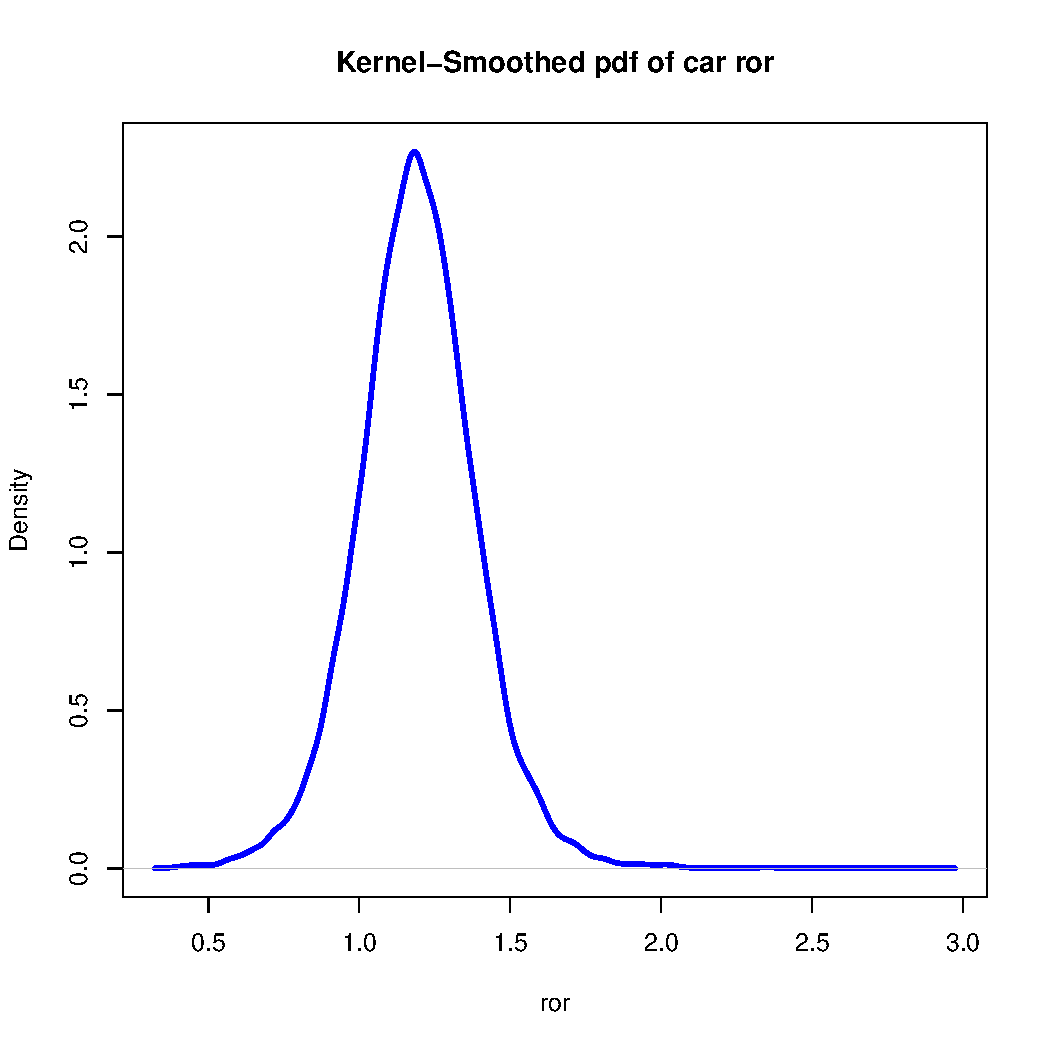
\includegraphics[scale = 0.5, keepaspectratio=true]{../Figures/density_ror}
  \caption{Probability Density Function of auctionl Prices} \label{fig:density_ror}
\end{figure}

\clearpage
%%%%%%%%%%%%%%%%%%%%%%%%%%%%%%%%%%%%%%%%

%%%%%%%%%%%%%%%%%%%%%%%%%%%%%%%%%%%%%%%%



\section{Data Visualization}

Begin with creating the variable age from the year variable, and taking in consideration that the data was gathered in 2020.

\subsection{Scatterplots of the data: pauc, pret, mileage, damage, ror, and cost}
%
\begin{figure}[h!]
  \centering
  \includegraphics[scale = 0.5, keepaspectratio=true]{../Figures/slpom_num_only}
  \caption{matrix of scatterplots} \label{fig:splom_num_only}
\end{figure}
% .
\clearpage

\subsection{considering adding some categorical variables: damage, dealer, }

\begin{figure}[h!]
  \centering
  \includegraphics[scale = 0.5, keepaspectratio=true]{../Figures/slpom_with_cat}
  \caption{considering dealer and age} \label{fig:splom_with_cat}
\end{figure}
\clearpage

\subsection{cheking the relationshp between mileage and age }

Figure \ref{fig:age_mileage_plot} showing the relationship between mileage and age 

\begin{figure}[h!]
  \centering
  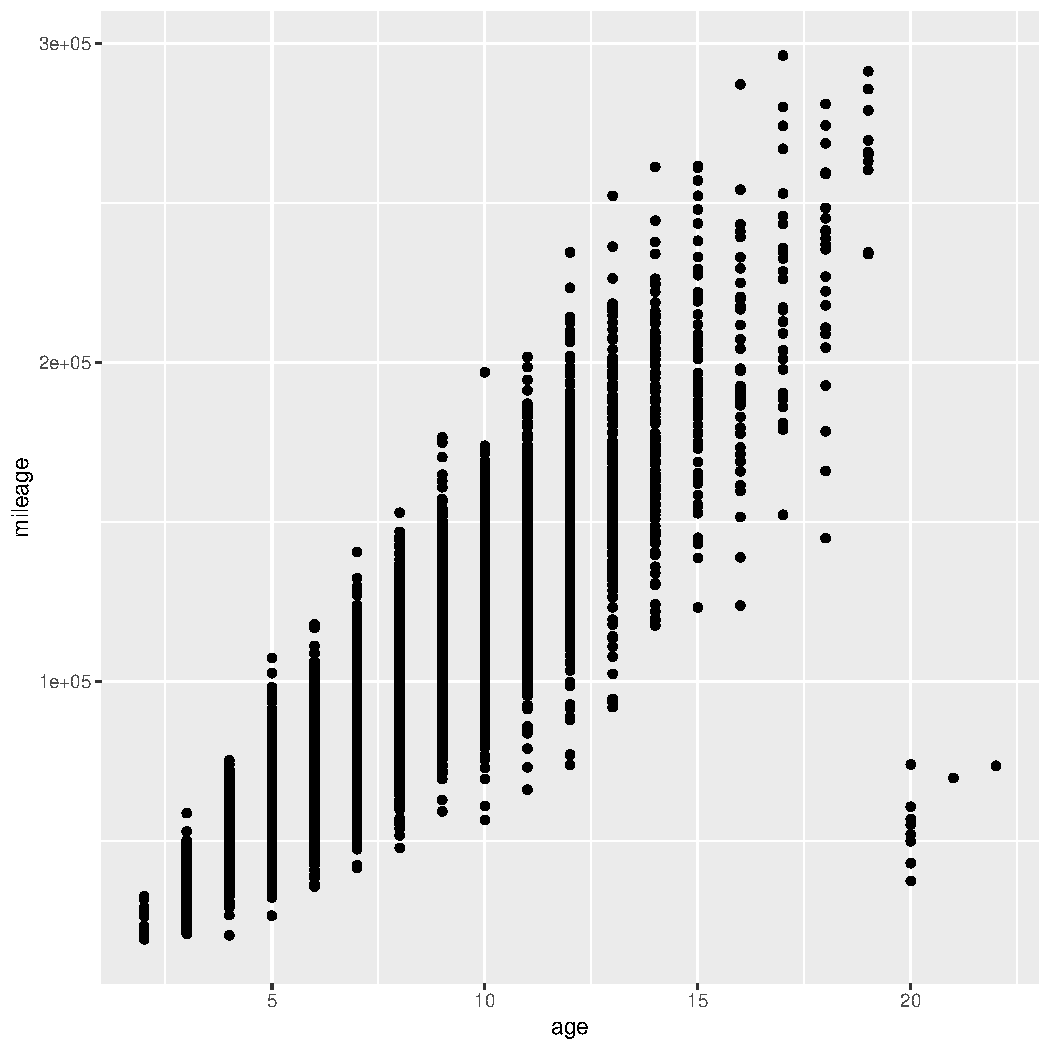
\includegraphics[scale = 0.5, keepaspectratio=true]{../Figures/age_mileage_plot}
  \caption{relationship between mileage and age} \label{fig:age_mileage_plot}
\end{figure}

\pagebreak
\subsection{cheking the relationship between pauc and age }




\begin{figure}[h!]
  \centering
  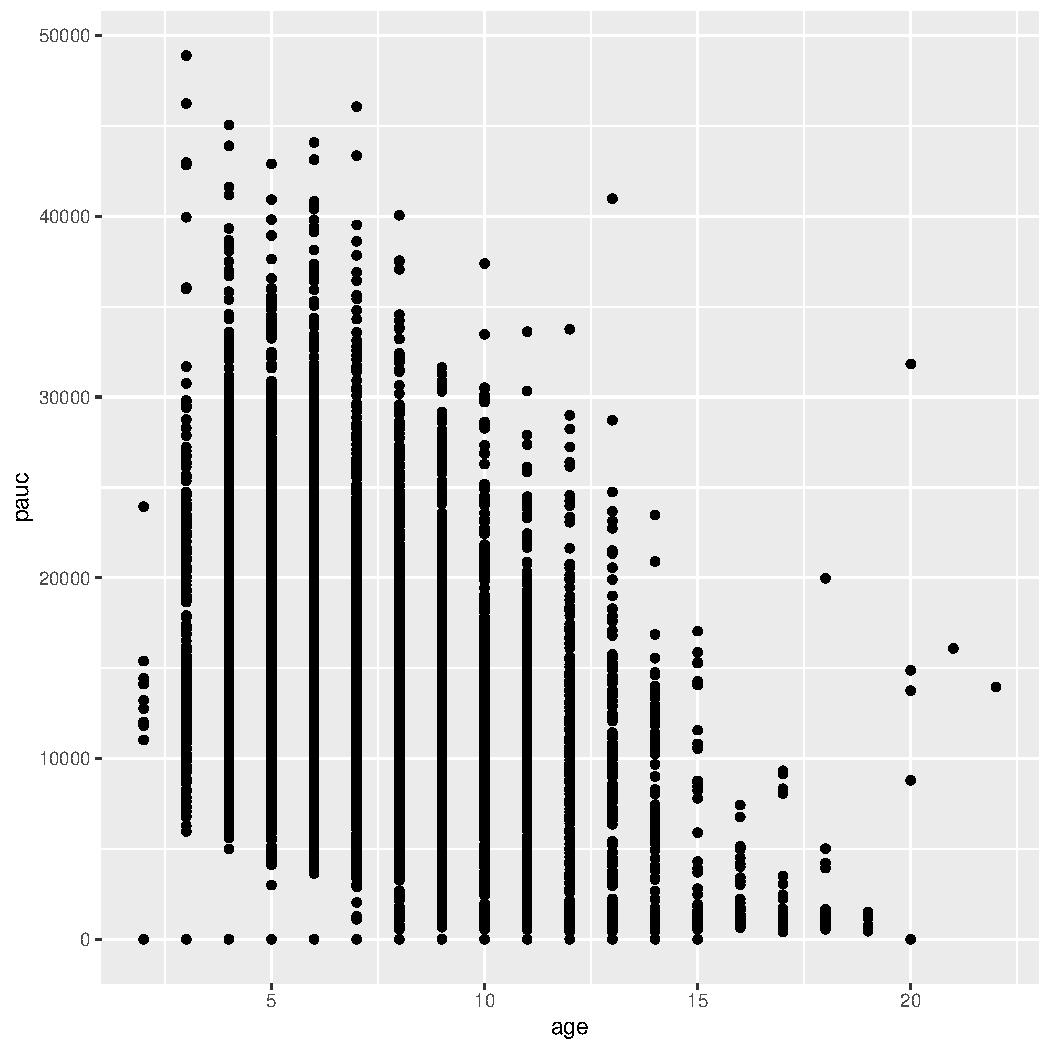
\includegraphics[scale = 0.5, keepaspectratio=true]{../Figures/pauc_age_plot}
  \caption{comparing the relationship between auction price and age} \label{fig:pauct_age_plot}
\end{figure}


\pagebreak

\subsection{cheking the relationship between pret and age }

\begin{figure}[h!]
  \centering
  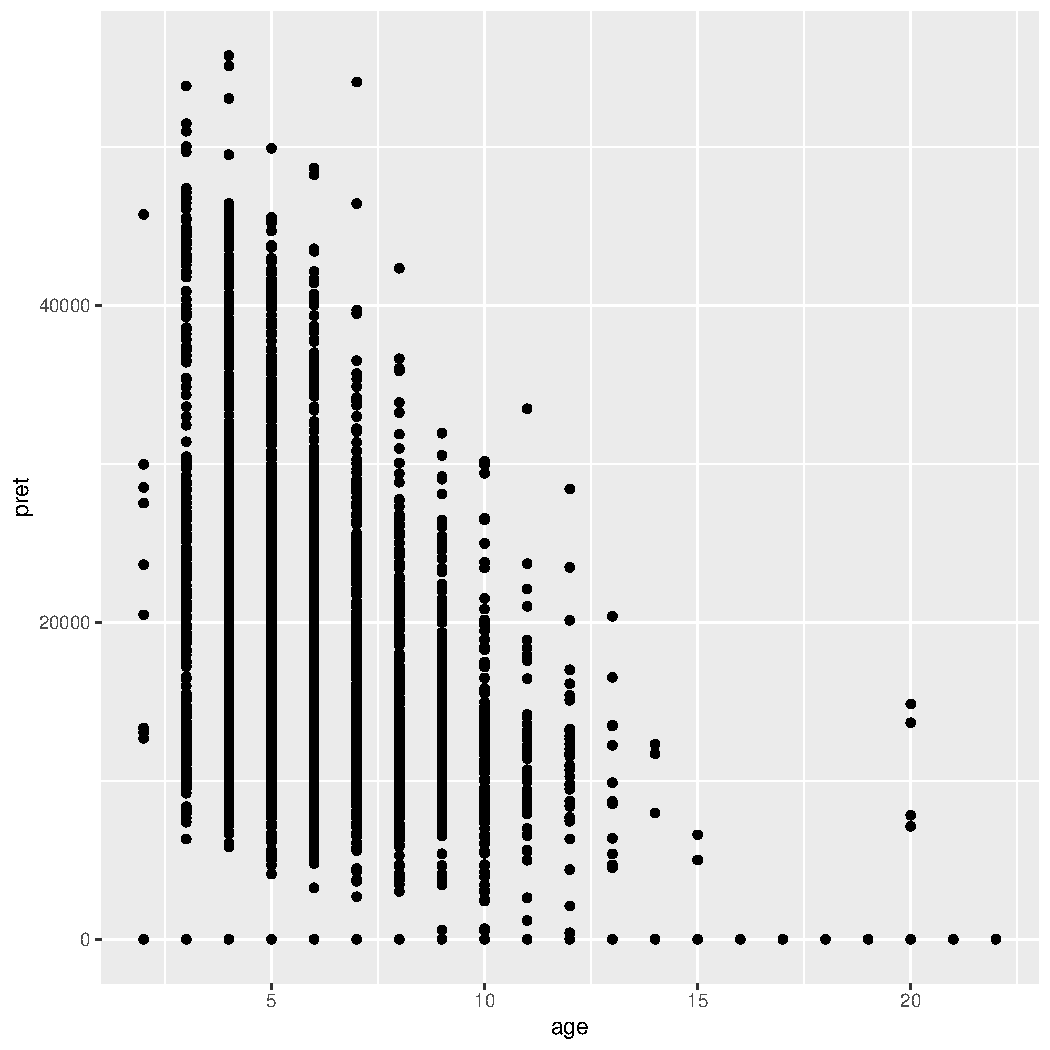
\includegraphics[scale = 0.5, keepaspectratio=true]{../Figures/pert_age_plot}
  \caption{comparing the relationship between auction price and age} \label{fig:pret_age_plot}
\end{figure}

\clearpage

%%%%%%%%%%%%%%%%%%%%%%%%%%%%%%%%%%%%%%%%
\section{Transforming The Dependent Variable}
\subsection{Probability Density Function of ror}

Figure \ref{fig:density_ror} shows  the kernel-smoothed probability density function of  ror.

\begin{figure}[h!]
  \centering
  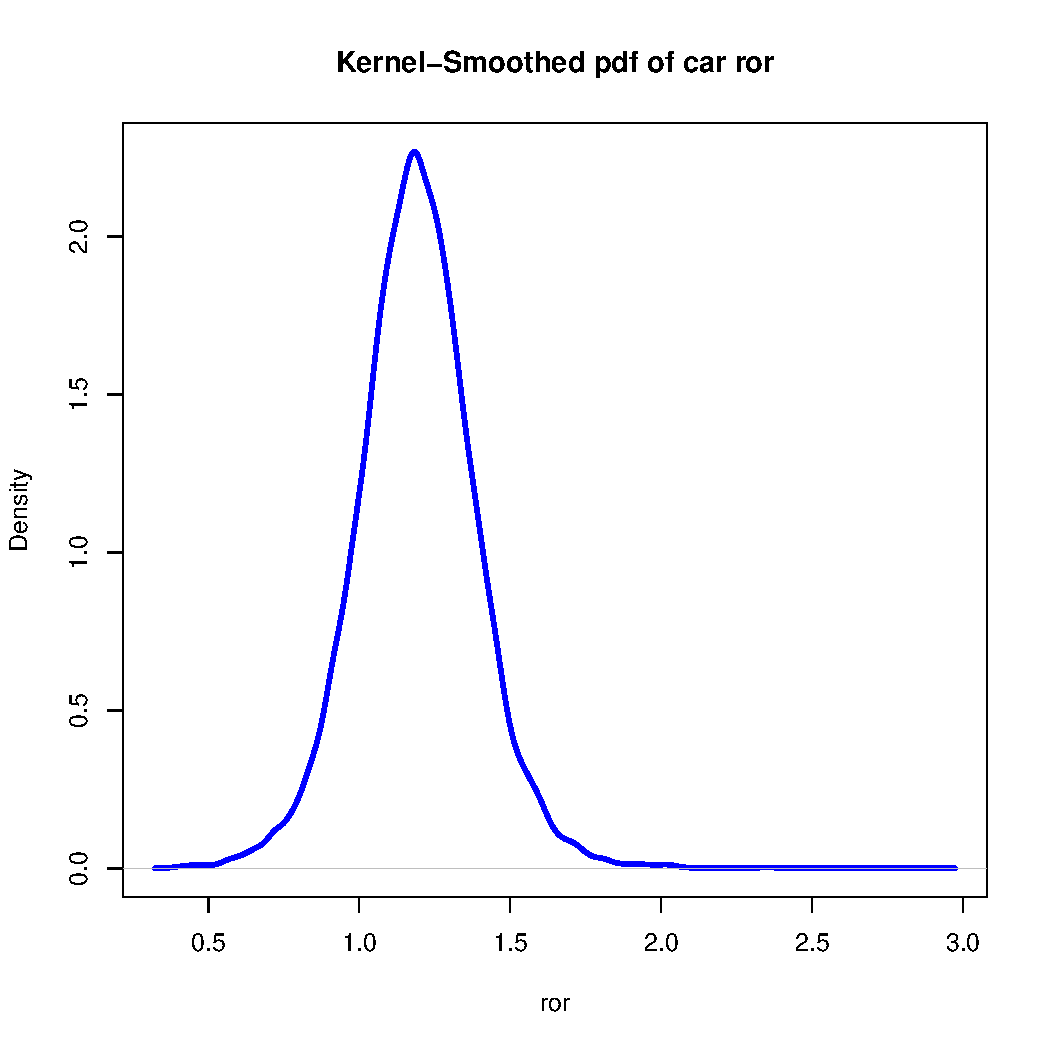
\includegraphics[scale = 0.5, keepaspectratio=true]{../Figures/density_ror}
  \caption{Probability Density Function of  ror} \label{fig:density_ror}
\end{figure}



\pagebreak
As a comparison, Figure \ref{fig:density_log_ror} shows the kernel-smoothed probability density function  of
ror.

\begin{figure}[h!]
  \centering
  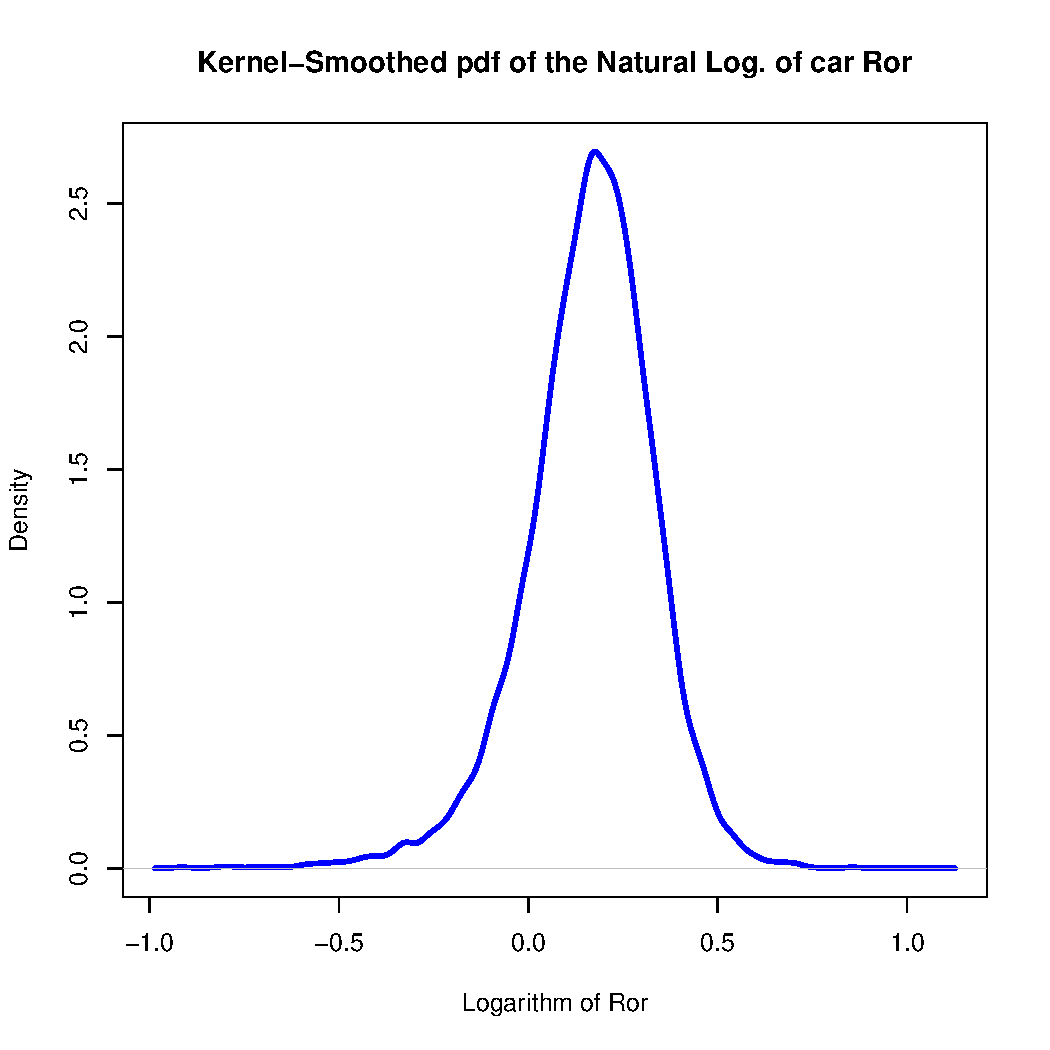
\includegraphics[scale = 0.5, keepaspectratio=true]{../Figures/density_log_ror}
  \caption{Probability Density Function of  ror} \label{fig:density_log_ror}
\end{figure}


\pagebreak
\subsection{Normality of the Original and Transformed Variables}

Figure \ref{fig:qq_ror} shows a pair of Q-Q plots, 
comparing quantiles of the empirical distribution against
the quantiles of the normal distribution. 
In the left panel, Figure \ref{subfig:qq_ror} shows this comparison 
for the original level of  ror, without transformation. 
In the right panel, Figure \ref{subfig:qq_log_ror} shows this comparison 
for the logarithmic transformation of  ror, without transformation. 
Consistent with the pair of distributions estimated above, 
each plot shows a divergence from a normal distribution,
suggesting that an optimal transformation might lie somewhere in the middle.
The Box-Cox transformation allows for this possibility. 

\begin{figure}[!ht]
\subfloat[ ror\label{subfig:qq_ror}]{%
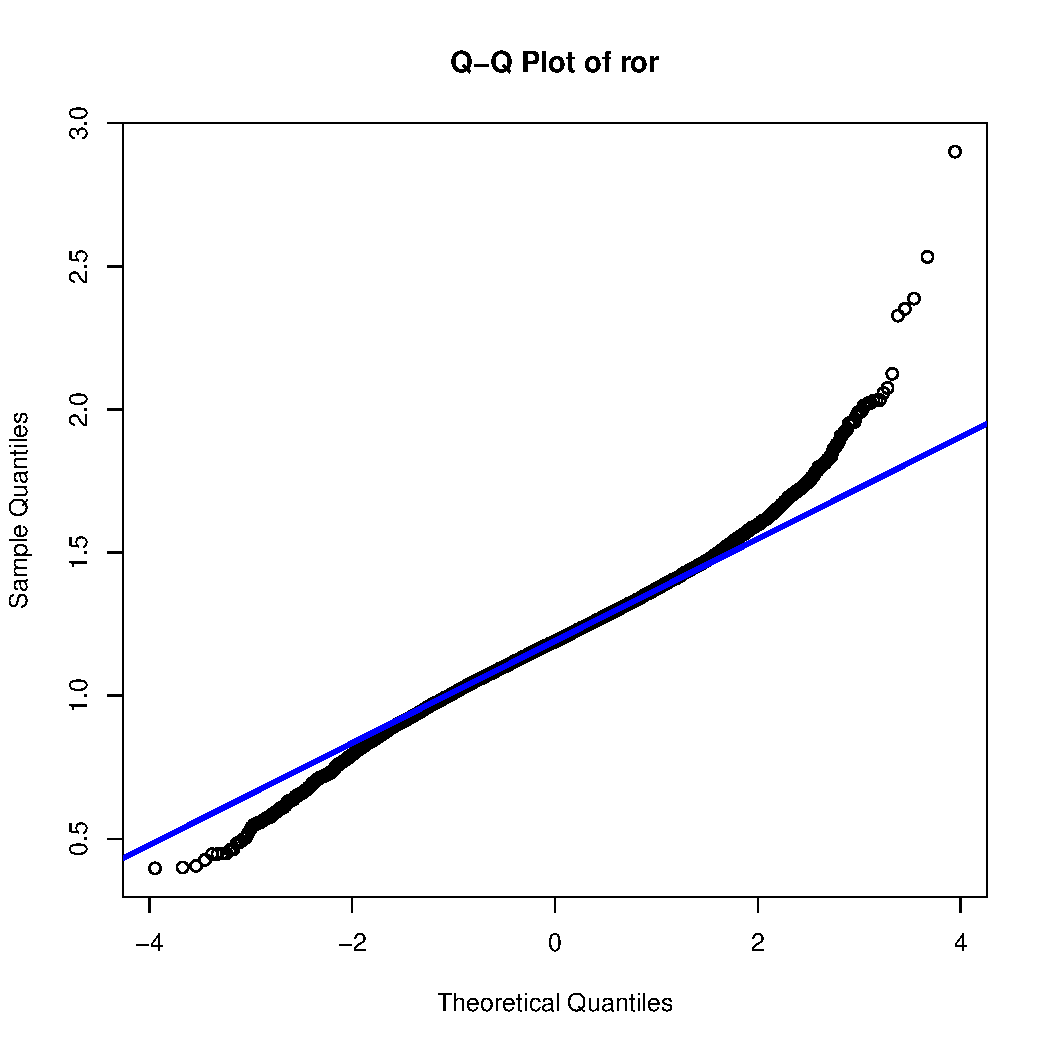
\includegraphics[width=0.5\textwidth]{../Figures/qq_ror}}
\hfill
\subfloat[Transformed  ror\label{subfig:qq_log_ror}]{%
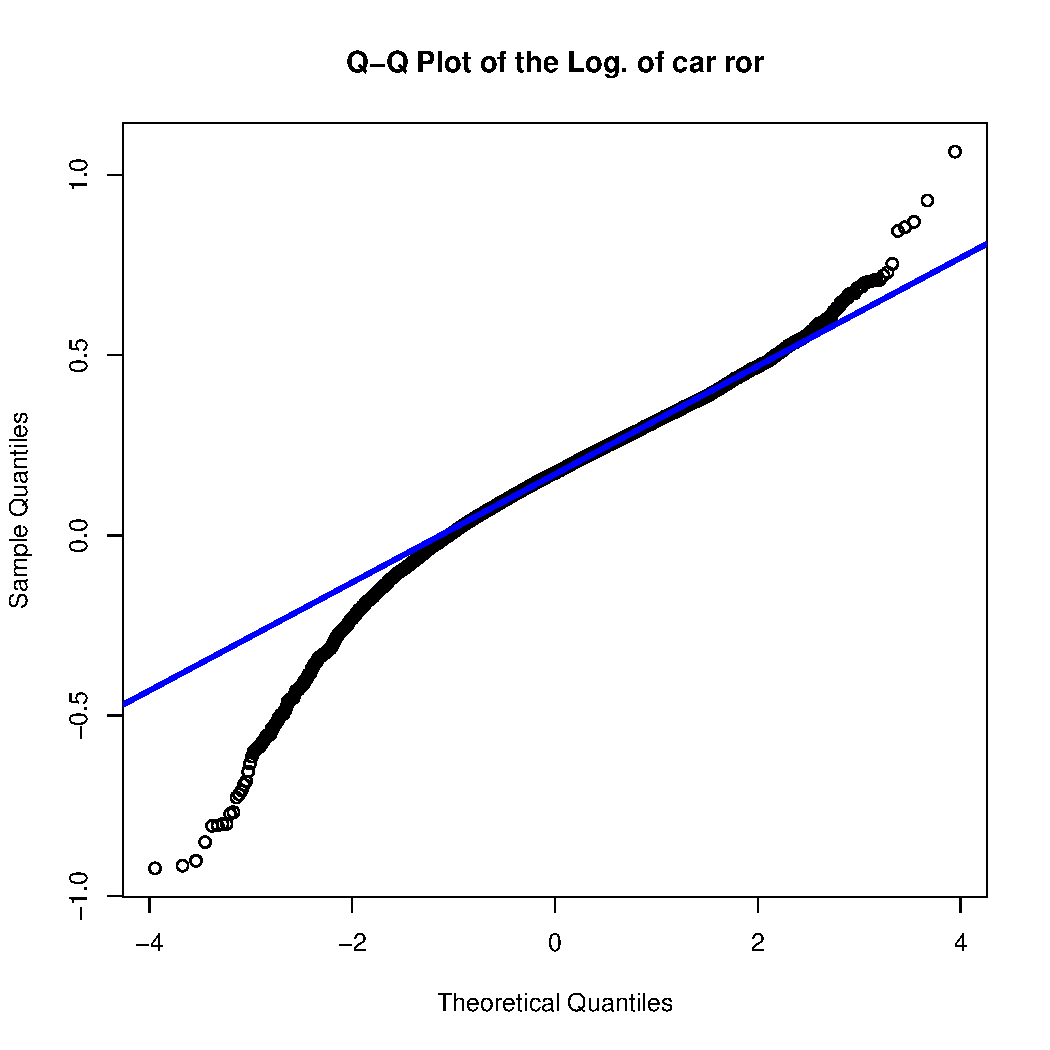
\includegraphics[width=0.5\textwidth]{../Figures/qq_log_ror}}

\caption{Q-QPlots of the Log. and Levels of Ror}
\label{fig:qq_ror}
\end{figure}

\pagebreak
\clearpage

\subsection{Box-Cox Transformation of  ror}

Under the Box--Cox transformation of $P_n$, Ror $n$
is calculated as follows,
$$\Lambda(P_n)\equiv
  \begin{cases}
	\frac{P_n^\lambda-1}{\lambda}	& \textrm{if } \lambda > 0 \\
           \log P_n                     			& \textrm{if } \lambda = 0.\\
  \end{cases}
$$
The following code block defines a function that performs a
Box-Cox transformation.

\vspace{1.0in}







\begin{lstlisting}[language=R]
# Box-Cox transformation.
Lambda_Price <- function(price, lambda) {
  if (lambda == 0) {
    return(log(price))
  } else {
    return((price^lambda - 1)/lambda)
  }
}
\end{lstlisting}

\pagebreak
\subsection{Log-likelihood Function}

Under the Box-Cox transformation,
the fly reel prices can be decomposed into a location parameter $\mu^0$ 
and an error $U$, so
$$\Lambda(P_n) = \mu^0(\lambda) + U_n,$$
where the $U_n$s are independent, mean-zero, constant-variance 
$\sigma^2(\lambda)$, Gaussian (normal) errors. 
In the above equation, for clarity, the dependence of $\mu^0$ and 
$\sigma^2(\lambda)$ on $\lambda$ is made explicit.


The next code block defines a likelihood function for the normal distribution of the errors
as a function of the parameter $\lambda$.






\begin{lstlisting}[language=R]
log_like_uni <- function(ror, lambda) {

  # Calculate maximum likelighood estimates of the parameters.
  n <- length(ror)
  lambda_ror <- Lambda_ror(price, lambda)
  mu_0_lambda <- mean(lambda_ror)
  sigma_2_lambda <- sum((lambda_ror - mu_0_lambda)^2)/n

  # Calculate the log-likelihood from the sum of the logarithms
  # of the density of the normal distribution.
  like <- - n/2*log(2*pi*sigma_2_lambda)
  like <- like - 1/2/sigma_2_lambda*sum((lambda_ror - mu_0_lambda)^2)
  like <- like + (lambda - 1)*sum(log(ror))
  return(like)
}
\end{lstlisting}

\pagebreak

As a first approximation, 
One can calculate the value of the log-likelihood function on a grid of values
to find an optimal value of $\lambda$.
The plot of this likelihood function is shown in Figure \ref{fig:box_cox_loglike_uni}.
The red points represent the values of the log-likelihood 
at the optimum $\lambda = 0.43$ and at $\lambda = 0$ and $\lambda = 1$.

\begin{lstlisting}[language=R]
# Calculate values of the log-likelihood function.
lambda_grid <- seq(-1, 2.5, by = 0.001)
like_grid <- 0*lambda_grid
for (lambda_num in 1:length(lambda_grid)) {
  like_grid[lambda_num] <- log_like_uni(ror = Truck[, 'ror'],
                                    lambda = lambda_grid[lambda_num])
}
\end{lstlisting}

\begin{figure}[h!]
  \centering
  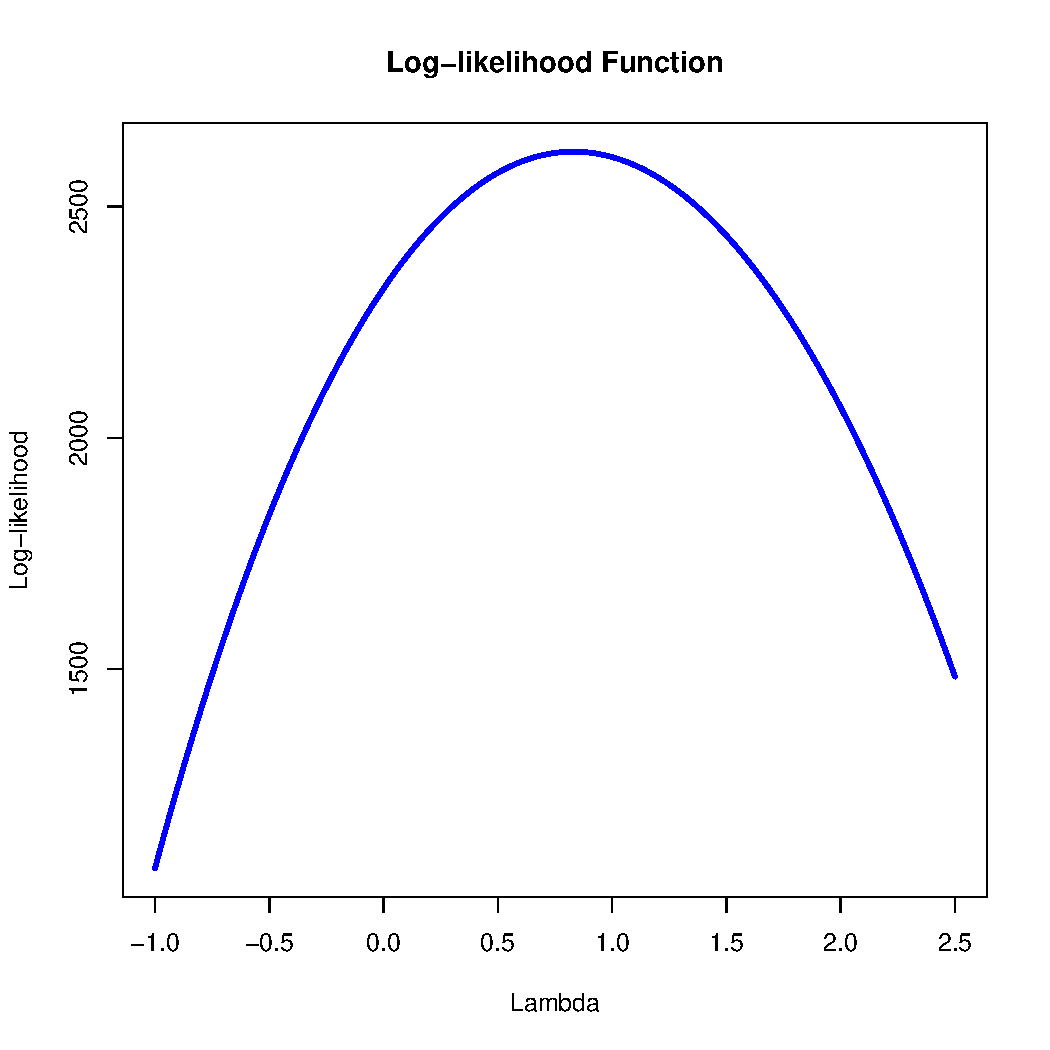
\includegraphics[scale = 0.5, keepaspectratio=true]{../Figures/box_cox_loglike_uni}
  \caption{Log-likelihood Function for Box-Cox Transformation} \label{fig:box_cox_loglike_uni}
\end{figure}


\pagebreak
\pagebreak
\subsection{Testing for an Appropriate Transformation}

Now we consider the statistical properties of these estimates
by calculating a likelihood ratio statistic.

\begin{lstlisting}[language=R]
> # Calculate likelihood ratio statistics.
> LR_stat_0 <- - 2*(like_mu_0 - like_MLE)
> print(LR_stat_0)
[1] 11.76066
> LR_stat_1 <- - 2*(like_mu_1 - like_MLE)
> print(LR_stat_1)
[1] 2.937618
> 
> 
> # Compare to quantile of chi-squared distribution with 1 degree of freedom.
> LR_cv_5 <- qchisq(p = 0.95, df = 1)
> print(LR_cv_5)
[1] 3.841459
> 
> # Calculate p-values for these tests.
> p_value_0 <- 1 - pchisq(q = LR_stat_0, df = 1)
> print(p_value_0)
[1] 0.0006049
> p_value_1 <- 1 - pchisq(q = LR_stat_1, df = 1)
> print(p_value_1)
[1] 0.08653825
> 
\end{lstlisting}

Statistically, this is evidence to reject them both.
This suggests using the transformation at the MLE.
However, one may want to investigate further 
to find out whether it is worth 
transforming the data. 
There exists a trade-of between interpretability and 
the accuracy of the statistical specification. 


\clearpage

\subsection{\textsf{R} Packages for the Box-Cox Transformation}
\subsection*{Using the \texttt{MASS} Package}

As an illustration, we calculated
the likelihood ourselves.
However, there exist other packages
to output the estimation results for
an optimal Box-Cox transformation.

One option is to use the function from the \texttt{MASS} package.
This is an \textsf{R} package that accompanies a well-know statistics textbook
and has a great reputation. 
In the \texttt{MASS} package, the notation is the same as for a linear model.


\begin{lstlisting}[language=R]
# In the MASS package, the notation is the same as for a linear model.
# i.e., summary(lm(ror ~ 1, data = DF))
bc_grid_MASS <- MASS::boxcox(ror ~ 1,
                             data = DF,
                             lambda = lambda_grid)
\end{lstlisting}

The output is plotted in Figure \ref{fig:plot_like_MASS}.

\begin{figure}[h!]
  \centering
  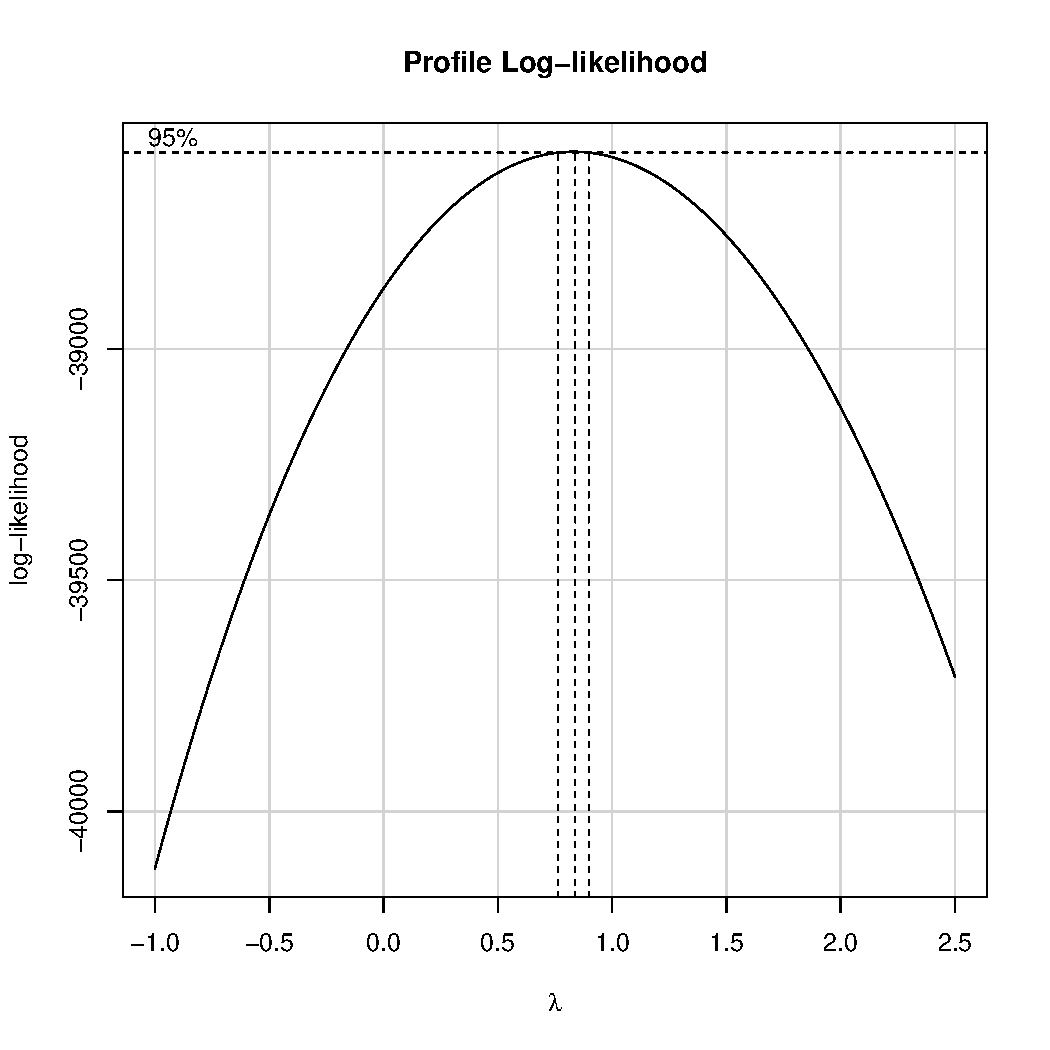
\includegraphics[scale = 0.5, keepaspectratio=true]{../Figures/plot_like_MASS}
  \caption{Log-likelihood Function for Box-Cox Transformation (\texttt{MASS} package)} \label{fig:plot_like_MASS}
\end{figure}


\clearpage

%%%%%%%%%%%%%%%%%%%%%%%%%%%%%%%%%%%%%%%%
%%%%%%%%%%%%%%%%%%%%%%%%%%%%%%%%%%%%%%%%
\section{Linear Regression Models }
In this section we will go over a linear model which in clude quadratic specification
for mileage. 

The results of this regression specification are shown in 
Table \ref{tab:reg_sq_mileage}. 
% 

\begin{table}
\begin{center}
\begin{tabular}{l c}
\hline
 & Model 1 \\
\hline
(Intercept)         & $1.54122^{***}$  \\
                    & $(0.01503)$      \\
squared\_mileage    & $0.00000^{***}$  \\
                    & $(0.00000)$      \\
as.factor(make)2    & $0.00888$        \\
                    & $(0.00769)$      \\
as.factor(make)3    & $0.00754$        \\
                    & $(0.00825)$      \\
as.factor(make)4    & $0.00796$        \\
                    & $(0.00678)$      \\
as.factor(make)5    & $0.00844$        \\
                    & $(0.00713)$      \\
as.factor(make)6    & $-0.04101^{***}$ \\
                    & $(0.00692)$      \\
as.factor(make)7    & $-0.03360^{***}$ \\
                    & $(0.00730)$      \\
as.factor(make)8    & $-0.07093^{***}$ \\
                    & $(0.01014)$      \\
as.factor(make)9    & $-0.06644^{***}$ \\
                    & $(0.01126)$      \\
as.factor(damage)2  & $-0.09296^{***}$ \\
                    & $(0.01219)$      \\
as.factor(damage)3  & $-0.12496^{***}$ \\
                    & $(0.01097)$      \\
as.factor(damage)4  & $-0.20366^{***}$ \\
                    & $(0.01105)$      \\
as.factor(damage)5  & $-0.18729^{***}$ \\
                    & $(0.01126)$      \\
as.factor(damage)6  & $-0.22644^{***}$ \\
                    & $(0.01143)$      \\
as.factor(damage)7  & $-0.30002^{***}$ \\
                    & $(0.01321)$      \\
as.factor(damage)8  & $-0.34428^{***}$ \\
                    & $(0.02169)$      \\
as.factor(damage)9  & $-0.33160^{***}$ \\
                    & $(0.02670)$      \\
as.factor(damage)10 & $-0.38087^{***}$ \\
                    & $(0.01568)$      \\
as.factor(dealer)2  & $-0.03230^{***}$ \\
                    & $(0.00949)$      \\
as.factor(dealer)3  & $0.05693^{***}$  \\
                    & $(0.00715)$      \\
as.factor(dealer)4  & $-0.05023^{***}$ \\
                    & $(0.00657)$      \\
as.factor(dealer)5  & $0.03503^{***}$  \\
                    & $(0.00902)$      \\
as.factor(dealer)6  & $-0.00188$       \\
                    & $(0.00641)$      \\
as.factor(dealer)7  & $0.02291^{**}$   \\
                    & $(0.00769)$      \\
as.factor(dealer)8  & $-0.04838^{***}$ \\
                    & $(0.00633)$      \\
as.factor(dealer)9  & $-0.05546^{***}$ \\
                    & $(0.00931)$      \\
mileage             & $-0.00000^{***}$ \\
                    & $(0.00000)$      \\
age                 & $-0.00315^{*}$   \\
                    & $(0.00139)$      \\
\hline
R$^2$               & $0.18143$        \\
Adj. R$^2$          & $0.17959$        \\
Num. obs.           & $12492$          \\
\hline
\multicolumn{2}{l}{\scriptsize{$^{***}p<0.001$; $^{**}p<0.01$; $^{*}p<0.05$}}
\end{tabular}
\caption{Quadratic Model for  ror}
\label{tab:reg_sq_damage}
\end{center}
\end{table}

% 
\clearpage
\subsection{Nonparametric Specification for Mileage}


The specification in 
Table \ref{tab:reg_sq_mileage}
assumes a quadratic functional form for
the relationship between ror and mileage. 
To consider the mileage variable alone, 
while accounting for the effects of other variables, 
one can fit a nonparametric model to the residuals 
from a model of ror, 
after regressing ror on the other variables. 
This leaves only the variation in ror that is not explained by the other variables. 
Going one step further, perform the same transformation to the mileage variable:
take the residuals from a model of mileage, 
after regressing mileage on the other variables. 
This allows a model that would fit exactly the same as if it were estimated within a full model with all variables included. 

The models shown in
Table \ref{tab:reg_sq_mileage_fwl}
illustrate this possibility. 
Model 1 is the original model in 
Table \ref{tab:reg_sq_mileage}. 
Model 2 is a regression omitting the mileage variables. 
Model 3 is a regression to predict mileage with the other explanatory variables in Model 2.
Finally, Model 4 shows the coefficients for mileage
from a regression of the residuals of Model 2
on the residuals from Model 3. 
Notice that these coefficients match those in Model 1. 
You might notice a slight difference in the standard errors, however, 
because these are calculated assuming coefficients 
for two variables, mileage and squared mileage,
rather than the full suite of ten parameters.
This equivalence of the coefficients can be used to fit
nonlinear models between a pair of variables by 
partialing out the effect of the other variables, 
using a mathematical result called the Frisch-Waugh-Lovell (FWL) theorem, 
maned after early statisticians and econometricians who used these methods. 


\begin{table}
\begin{center}
\begin{tabular}{l c c c c c}
\hline
 & Model 1 & Model 2 & Model 3 & Model 4 & Model 5 \\
\hline
(Intercept)       & $1.55532^{***}$  & $1.48921^{***}$  & $417.28353$         & $-7120046673.84860^{***}$ &                  \\
                  & $(0.01457)$      & $(0.01321)$      & $(787.39910)$       & $(287578978.10063)$       &                  \\
squared\_mileage  & $0.00000^{***}$  &                  &                     &                           &                  \\
                  & $(0.00000)$      &                  &                     &                           &                  \\
make2             & $0.00842$        & $0.00990$        & $110.05320$         & $190402292.75189$         &                  \\
                  & $(0.00744)$      & $(0.00749)$      & $(680.87770)$       & $(163120814.80287)$       &                  \\
make3             & $0.00969$        & $0.00976$        & $459.31099$         & $114623775.64120$         &                  \\
                  & $(0.00799)$      & $(0.00804)$      & $(731.29282)$       & $(175144161.20396)$       &                  \\
make4             & $0.00764$        & $0.00744$        & $1653.93328^{**}$   & $414586965.56382^{**}$    &                  \\
                  & $(0.00657)$      & $(0.00661)$      & $(600.84486)$       & $(143959825.49683)$       &                  \\
make5             & $0.00826$        & $0.00792$        & $178.27004$         & $85935326.39744$          &                  \\
                  & $(0.00690)$      & $(0.00695)$      & $(631.50117)$       & $(151283700.50529)$       &                  \\
make6             & $-0.04529^{***}$ & $-0.04427^{***}$ & $-189.71715$        & $71851502.06592$          &                  \\
                  & $(0.00670)$      & $(0.00675)$      & $(613.14388)$       & $(146912253.17325)$       &                  \\
make7             & $-0.03770^{***}$ & $-0.03772^{***}$ & $232.73905$         & $31089322.48710$          &                  \\
                  & $(0.00707)$      & $(0.00712)$      & $(646.74458)$       & $(154960733.32422)$       &                  \\
make8             & $-0.07169^{***}$ & $-0.06526^{***}$ & $-1116.68863$       & $405468029.64154$         &                  \\
                  & $(0.00982)$      & $(0.00987)$      & $(897.06345)$       & $(214957186.41487)$       &                  \\
make9             & $-0.06409^{***}$ & $-0.05747^{***}$ & $-1456.63485$       & $289356844.48372$         &                  \\
                  & $(0.01090)$      & $(0.01096)$      & $(996.40072)$       & $(238712493.31898)$       &                  \\
damage2           & $-0.11601^{***}$ & $-0.12052^{***}$ &                     & $-477557264.95650$        &                  \\
                  & $(0.01183)$      & $(0.01190)$      &                     & $(259105343.95793)$       &                  \\
damage3           & $-0.16372^{***}$ & $-0.17049^{***}$ &                     & $-525186237.05704^{*}$    &                  \\
                  & $(0.01071)$      & $(0.01077)$      &                     & $(234420390.55166)$       &                  \\
damage4           & $-0.25179^{***}$ & $-0.25950^{***}$ &                     & $-198173573.25832$        &                  \\
                  & $(0.01083)$      & $(0.01088)$      &                     & $(236976024.12451)$       &                  \\
damage5           & $-0.23679^{***}$ & $-0.24454^{***}$ &                     & $94100014.61171$          &                  \\
                  & $(0.01104)$      & $(0.01110)$      &                     & $(241679119.26264)$       &                  \\
damage6           & $-0.28664^{***}$ & $-0.29541^{***}$ &                     & $292839776.13712$         &                  \\
                  & $(0.01127)$      & $(0.01132)$      &                     & $(246513338.77132)$       &                  \\
damage7           & $-0.36724^{***}$ & $-0.37952^{***}$ &                     & $1534425773.03473^{***}$  &                  \\
                  & $(0.01301)$      & $(0.01305)$      &                     & $(284113106.61901)$       &                  \\
damage8           & $-0.41161^{***}$ & $-0.42590^{***}$ &                     & $4757613321.06478^{***}$  &                  \\
                  & $(0.02113)$      & $(0.02116)$      &                     & $(460833981.58933)$       &                  \\
damage9           & $-0.39495^{***}$ & $-0.40004^{***}$ &                     & $4530087626.13372^{***}$  &                  \\
                  & $(0.02595)$      & $(0.02606)$      &                     & $(567384547.76183)$       &                  \\
damage10          & $-0.44599^{***}$ & $-0.42566^{***}$ &                     & $12141646912.63641^{***}$ &                  \\
                  & $(0.01535)$      & $(0.01443)$      &                     & $(314119938.87532)$       &                  \\
dealer2           & $-0.03791^{***}$ & $-0.03691^{***}$ & $-1410.07372$       & $-255222858.23687$        &                  \\
                  & $(0.00919)$      & $(0.00925)$      & $(840.54273)$       & $(201424339.62329)$       &                  \\
dealer3           & $0.05242^{***}$  & $0.05477^{***}$  & $287.92384$         & $-252658058.52460$        &                  \\
                  & $(0.00693)$      & $(0.00697)$      & $(630.47152)$       & $(151792533.58411)$       &                  \\
dealer4           & $-0.05643^{***}$ & $-0.05417^{***}$ & $-1005.82544$       & $84804145.63787$          &                  \\
                  & $(0.00637)$      & $(0.00641)$      & $(578.74384)$       & $(139470199.73761)$       &                  \\
dealer5           & $0.03791^{***}$  & $0.03730^{***}$  & $498.50283$         & $-272544391.03262$        &                  \\
                  & $(0.00874)$      & $(0.00880)$      & $(798.43020)$       & $(191544613.63839)$       &                  \\
dealer6           & $0.00365$        & $0.00285$        & $221.93701$         & $-70597546.76223$         &                  \\
                  & $(0.00621)$      & $(0.00625)$      & $(568.26343)$       & $(136169915.72600)$       &                  \\
dealer7           & $0.03135^{***}$  & $0.03054^{***}$  & $159.07665$         & $-513899436.51786^{**}$   &                  \\
                  & $(0.00746)$      & $(0.00750)$      & $(680.10670)$       & $(163356357.02883)$       &                  \\
dealer8           & $-0.05479^{***}$ & $-0.05145^{***}$ & $-1971.19980^{***}$ & $-65831910.69756$         &                  \\
                  & $(0.00614)$      & $(0.00617)$      & $(557.10270)$       & $(134411749.28556)$       &                  \\
dealer9           & $-0.06341^{***}$ & $-0.06346^{***}$ & $-511.03343$        & $-26484745.78757$         &                  \\
                  & $(0.00902)$      & $(0.00908)$      & $(823.92188)$       & $(197621661.82632)$       &                  \\
mileage           & $-0.00000^{***}$ &                  &                     &                           &                  \\
                  & $(0.00000)$      &                  &                     &                           &                  \\
age               & $-0.00314^{*}$   & $-0.01415^{***}$ & $12084.52582^{***}$ & $2212445074.10095^{***}$  &                  \\
                  & $(0.00135)$      & $(0.00070)$      & $(57.45278)$        & $(15294578.10953)$        &                  \\
type1             & $0.10347^{***}$  & $0.09882^{***}$  & $4085.76380^{***}$  & $358274580.13725^{***}$   &                  \\
                  & $(0.00359)$      & $(0.00360)$      & $(315.78201)$       & $(78355276.64345)$        &                  \\
mileage\_resid    &                  &                  &                     &                           & $-0.00000^{***}$ \\
                  &                  &                  &                     &                           & $(0.00000)$      \\
mileage\_2\_resid &                  &                  &                     &                           & $0.00000^{***}$  \\
                  &                  &                  &                     &                           & $(0.00000)$      \\
\hline
R$^2$             & $0.23248$        & $0.22213$        & $0.82763$           & $0.80355$                 & $0.00979$        \\
Adj. R$^2$        & $0.23070$        & $0.22044$        & $0.82738$           & $0.80312$                 & $0.00963$        \\
Num. obs.         & $12492$          & $12492$          & $12492$             & $12492$                   & $12492$          \\
\hline
\multicolumn{6}{l}{\scriptsize{$^{***}p<0.001$; $^{**}p<0.01$; $^{*}p<0.05$}}
\end{tabular}
\caption{Quadratic Model for ROR: FWL Regressions}
\label{tab:reg_sq_mileage_fwl}
\end{center}
\end{table}


\pagebreak 
To illustrate the fit of the model, 
Figure \ref{fig:dev_vs_mileage} shows a scatter plot 
of the residual ror on mileage. 
The observations are shown in blue
and the fitted values are shown in red.
The variation in the fitted values results from the 
fact that it is not plotted against the transformed excess mileage variable used in the regressions.


\begin{figure}[h!]
  \centering
  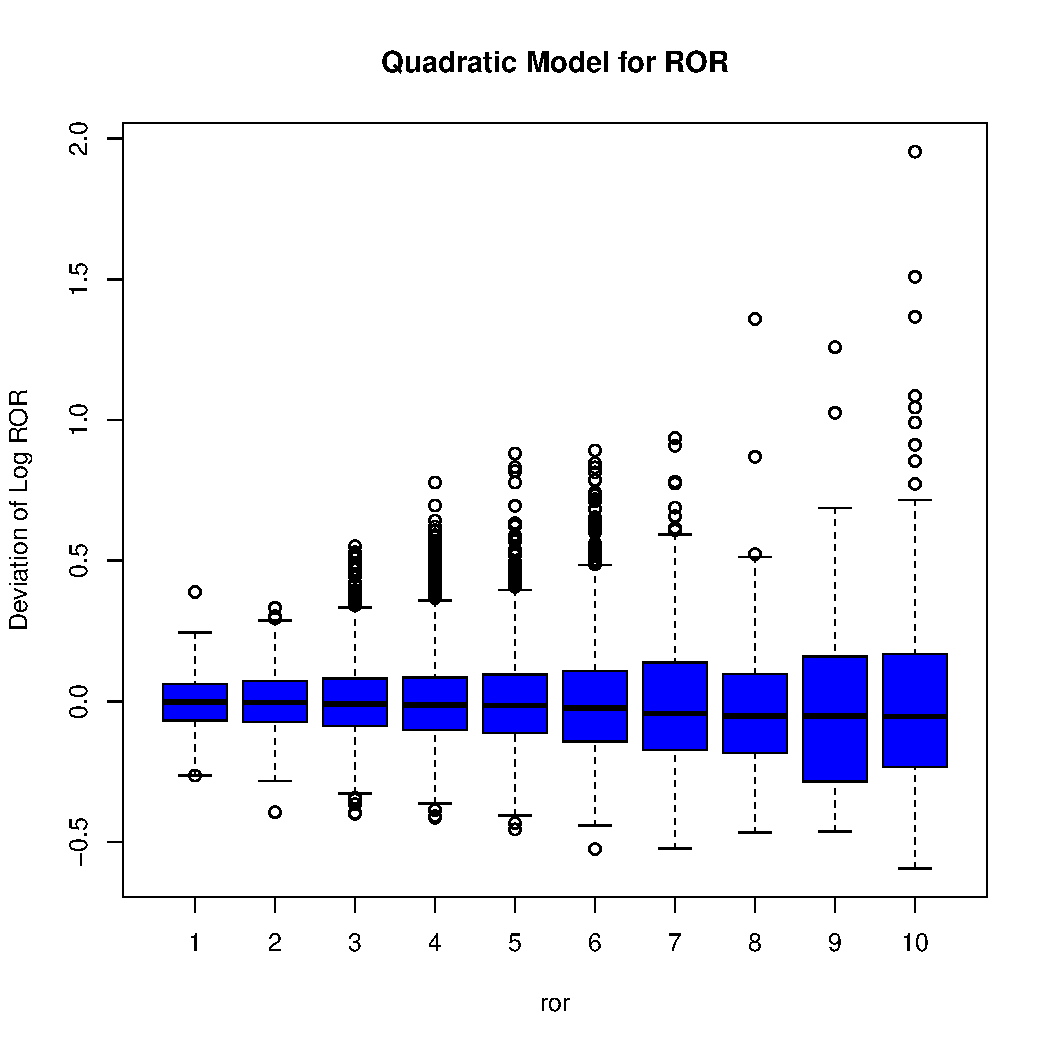
\includegraphics[scale = 0.5, keepaspectratio=true]{../Figures/dev_vs_ror}
  \caption{Linear-Quadratic Model for ROR} \label{fig:dev_vs_ror}
\end{figure}







%%%%%%%%%%%%%%%%%%%%%%%%%%%%%%%%%%%%%%%%
%%%%%%%%%%%%%%%%%%%%%%%%%%%%%%%%%%%%%%%%
\section{Transforming the Explanatory Variables}

\subsection{The Box--Tidwell Transformation}

The Box--Tidwell function tests for non-linear relationships
to the mean of the dependent variable.
The nonlinearity is in the form of an
exponential transformation in the form of the Box-Cox
transformation, except that the transformation is taken
on the explanatory variables.


\subsection{Transformation of mileage}


Performing the transformation on the mileage variable
produces a modified form of the linear model.
This specification allows a single exponential
transformation on mileage, rather than a quadratic form.

\begin{verbatim} MLE of lambda Score Statistic (z)  Pr(>|z|)    
      -0.36799              10.036 < 2.2e-16 ***
---
Signif. codes:  0 �***� 0.001 �**� 0.01 �*� 0.05 �.� 0.1 � � 1

iterations =  10 
\end{verbatim}

The \textsf{R} output is the statistics for a test of nonlinearity:
that the exponent $\lambda$ in the Box--Tidwell transformation is zero.
%
The "\texttt{MLE of lambda}" statistic is the optimal exponent on mileage.
Similar to the Box-Cox transformation,
with Box-Tidwell, the exponents are on the explanatory variables
and are all called lambda, in contrast
to the parameter $\tau$ in our class notes.
The exponent is significantly different from 0,
although it is a small positive value,
which suggests an increasing relationship
for the value of mileage
with a slope that is sharply declining.
Next I consider the possibility of a changing relationship 
for the next continuous variable. 


\subsection{Transformation of Age}


\begin{verbatim} MLE of lambda Score Statistic (z) Pr(>|z|)
     -0.089943              1.3022   0.1928

iterations =  24 
\end{verbatim}

This coefficient is effectively 1, which is more evidence of
a purely linear relationship between \texttt{log\_ror}
and age: the percentage depreciation rate is constant.
Next, I will consider the possibility of nonlinearity 
in depreciation from cost. 

\subsection{Transformation of cost}


\begin{verbatim} MLE of lambda Score Statistic (z)  Pr(>|z|)    
       0.77872             -4.6859 2.787e-06 ***
---
Signif. codes:  0 �***� 0.001 �**� 0.01 �*� 0.05 �.� 0.1 � � 1

iterations =  2 
\end{verbatim}

Although $\hat{\lambda}$ is not statistically significant,
this suggests a moderately increasing relationship
between the ror and cost,
which means that car with high cost
will generate low ror

Since a nonlinear relationship was detected with mileage,
I will next estimate a model
with nonlinearity in all three continuous variables.


\subsection{Transformation of All Three Continuous Variables}





The performance is similar to the other models with
forms of nonlinearity for the value of mileage.
Now consider the full set of such models in a table for a final comparison.


\pagebreak
\section{Final Comparison of Candidate Models}

I created one more variable \texttt{mileage\_bt}
by raising mileage to the optimal exponent 
$\hat{\lambda} = 0.1143693$. 
Then, I included this variable in the place of 
the mileage variables a the linear regression model.
% 
collects the results
of the set of models from the three forms of nonlinearity.
Model 1 is the linear regression model with 
a quadratic form for horsepower. 
Model 2 is the semiparametric model with
a nonparametric form for horsepower. 
Model 3 has the same specification as the other two, 
except that the mileage variable is transformed using the optimal
exponent for the Box-Tidwell transformation. 
% 
The last model has the highest R-squared
among the ones we have estimated.
Again, the differences are marginal, so the practical recommendation
is the model with the quadratic relationship for mileage, 
which has a simpler interpretation.
 


\clearpage
%%%%%%%%%%%%%%%%%%%%%%%%%%%%%%%%%%%%%%%%
%%%%%%%%%%%%%%%%%%%%%%%%%%%%%%%%%%%%%%%%
\section{Sample Selection Model }
\subsubsection{Separate Models by type of sales}
%%%%%%%%%%%%%%%%%%%%%%%%%%%%%%%%%%%%%%%%
we can check which type of sales will produce more return 
 
Table \ref{tab:reg_type}
shows the estimates for two separate models
by type of salesr.
%
Model 1 shows the estimates for 
the full sample,
Model 2 shows the estimates from the full model for 
retail sales
and Model 3
shows reduced model for retail sales. 
% 
Models 4 and 5 show the estimates from a full and reduced version of auction sales.
 
% 



\begin{table}
\begin{center}
\begin{tabular}{l c}
\hline
 & Model 1 \\
\hline
(Intercept)         & $1.54122^{***}$  \\
                    & $(0.01503)$      \\
squared\_mileage    & $0.00000^{***}$  \\
                    & $(0.00000)$      \\
as.factor(make)2    & $0.00888$        \\
                    & $(0.00769)$      \\
as.factor(make)3    & $0.00754$        \\
                    & $(0.00825)$      \\
as.factor(make)4    & $0.00796$        \\
                    & $(0.00678)$      \\
as.factor(make)5    & $0.00844$        \\
                    & $(0.00713)$      \\
as.factor(make)6    & $-0.04101^{***}$ \\
                    & $(0.00692)$      \\
as.factor(make)7    & $-0.03360^{***}$ \\
                    & $(0.00730)$      \\
as.factor(make)8    & $-0.07093^{***}$ \\
                    & $(0.01014)$      \\
as.factor(make)9    & $-0.06644^{***}$ \\
                    & $(0.01126)$      \\
as.factor(damage)2  & $-0.09296^{***}$ \\
                    & $(0.01219)$      \\
as.factor(damage)3  & $-0.12496^{***}$ \\
                    & $(0.01097)$      \\
as.factor(damage)4  & $-0.20366^{***}$ \\
                    & $(0.01105)$      \\
as.factor(damage)5  & $-0.18729^{***}$ \\
                    & $(0.01126)$      \\
as.factor(damage)6  & $-0.22644^{***}$ \\
                    & $(0.01143)$      \\
as.factor(damage)7  & $-0.30002^{***}$ \\
                    & $(0.01321)$      \\
as.factor(damage)8  & $-0.34428^{***}$ \\
                    & $(0.02169)$      \\
as.factor(damage)9  & $-0.33160^{***}$ \\
                    & $(0.02670)$      \\
as.factor(damage)10 & $-0.38087^{***}$ \\
                    & $(0.01568)$      \\
as.factor(dealer)2  & $-0.03230^{***}$ \\
                    & $(0.00949)$      \\
as.factor(dealer)3  & $0.05693^{***}$  \\
                    & $(0.00715)$      \\
as.factor(dealer)4  & $-0.05023^{***}$ \\
                    & $(0.00657)$      \\
as.factor(dealer)5  & $0.03503^{***}$  \\
                    & $(0.00902)$      \\
as.factor(dealer)6  & $-0.00188$       \\
                    & $(0.00641)$      \\
as.factor(dealer)7  & $0.02291^{**}$   \\
                    & $(0.00769)$      \\
as.factor(dealer)8  & $-0.04838^{***}$ \\
                    & $(0.00633)$      \\
as.factor(dealer)9  & $-0.05546^{***}$ \\
                    & $(0.00931)$      \\
mileage             & $-0.00000^{***}$ \\
                    & $(0.00000)$      \\
age                 & $-0.00315^{*}$   \\
                    & $(0.00139)$      \\
\hline
R$^2$               & $0.18143$        \\
Adj. R$^2$          & $0.17959$        \\
Num. obs.           & $12492$          \\
\hline
\multicolumn{2}{l}{\scriptsize{$^{***}p<0.001$; $^{**}p<0.01$; $^{*}p<0.05$}}
\end{tabular}
\caption{Quadratic Model for  ror}
\label{tab:reg_sq_damage}
\end{center}
\end{table}


\clearpage


%%%%%%%%%%%%%%%%%%%%%%%%%%%%%%%%%%%%%%%%
%%%%%%%%%%%%%%%%%%%%%%%%%%%%%%%%%%%%%%%%
\section{Summary}
The sample selection model that was best for the variables is show below. The
model was created by sampling the auction and retail data within the data set.
Different models were played with but to show all the variables on one table,
only the final one was shown as it created multiple lines due to dealer being
a categorical variable and creating multiple lines. The retail sample model excluded the mileage, square root of mileage and make variables while the auction
excluded the mileage and make variables.
The sample model ended up with all the variables being signficant including the
different types of dealers between auction and retail. Comparitevly only dealer
6 within the auction data set for the linear model was not signficant while the
other dealers were. This could mean that dealer is not as important to some
people buying at the auction sales. The age variable coefficient for retail in
the sample model was -0.02 while in the linear model it was -0.004. This could
show that age has more of an impact in the retail sales than was shown in the
linear model. On the other hand, the sample model age variable coefficient was
-0.0045 compared to a -0.0058. This is a much smaller increase between the
models when compared to the difference in retail age differences. It could be
considered that people selling in retail should be more wary of the age of cars
sold as it can lower the rate of return for the Used Trucks.
The differences in damage between the linear model and sample model were not
as huge. The auction coefficients for the sample was -0.078 versus the linear
model at -0.071. The retail coefficients for the sample were -0.098 and for the
linear it was -0.108. They both rose almost 0.007 and 0.01 respectively. These
is a tiny increase but it could be inferred that perhaps damage has more of an
impact on both retail and auction sales than was shown in the linear model.
The dealer variable also experiences some slight differences between the sample model and linear models. For the retail side, all the nine of the dealers
coefficients slightly increase from the linear model to the sample model which
would indicate that the dealers have a bigger impact on the rate of return. The
auction sales also had similar difference in that the sample model increased the
coefficient slightly when compared to the linear model.
Comparing the linear models from the split between the auction and retail
showed some differences in the r-squared. For auction, the r-squared was lowered from 0.41 to 0.39. However, the retail r-squared increased from 0.41 to 0.64.
This increased shows that the model had a better fit for the retail sales than the
auction sales. This could indicate that some of the variables within the model
may be more significant in retail than in auction and could be looked further to
see if reducing the model for auction could create a better linear model for the
auction data.
\clearpage


\begin{table}
\begin{center}
\begin{tabular}{l c c}
\hline
 & Model 1 & Model 2 \\
\hline
(Intercept)      & $-1.71363^{***}$ & $-0.55618^{***}$ \\
                 & $(0.13229)$      & $(0.03501)$      \\
squared\_mileage & $-0.00000$       &                  \\
                 & $(0.00000)$      &                  \\
make2            & $0.01770$        &                  \\
                 & $(0.05968)$      &                  \\
make3            & $-0.06942$       &                  \\
                 & $(0.06413)$      &                  \\
make4            & $0.00906$        &                  \\
                 & $(0.05284)$      &                  \\
make5            & $0.00534$        &                  \\
                 & $(0.05517)$      &                  \\
make6            & $0.13474^{*}$    &                  \\
                 & $(0.05382)$      &                  \\
make7            & $0.12964^{*}$    &                  \\
                 & $(0.05691)$      &                  \\
make8            & $0.02860$        &                  \\
                 & $(0.07649)$      &                  \\
make9            & $-0.05794$       &                  \\
                 & $(0.08431)$      &                  \\
damage2          & $0.68526^{***}$  &                  \\
                 & $(0.09773)$      &                  \\
damage3          & $1.08044^{***}$  &                  \\
                 & $(0.09008)$      &                  \\
damage4          & $1.32395^{***}$  &                  \\
                 & $(0.09074)$      &                  \\
damage5          & $1.35746^{***}$  &                  \\
                 & $(0.09227)$      &                  \\
damage6          & $1.71324^{***}$  &                  \\
                 & $(0.09454)$      &                  \\
damage7          & $2.16772^{***}$  &                  \\
                 & $(0.12167)$      &                  \\
damage8          & $2.77439^{***}$  &                  \\
                 & $(0.40744)$      &                  \\
damage9          & $2.12427^{***}$  &                  \\
                 & $(0.33546)$      &                  \\
damage10         & $2.66560^{***}$  &                  \\
                 & $(0.24264)$      &                  \\
dealer2          & $0.17120^{*}$    &                  \\
                 & $(0.07459)$      &                  \\
dealer3          & $0.17484^{**}$   &                  \\
                 & $(0.05965)$      &                  \\
dealer4          & $0.17479^{***}$  &                  \\
                 & $(0.05074)$      &                  \\
dealer5          & $-0.10854$       &                  \\
                 & $(0.07184)$      &                  \\
dealer6          & $-0.17649^{***}$ &                  \\
                 & $(0.04980)$      &                  \\
dealer7          & $-0.29420^{***}$ &                  \\
                 & $(0.06043)$      &                  \\
dealer8          & $0.18341^{***}$  &                  \\
                 & $(0.04895)$      &                  \\
dealer9          & $0.22319^{**}$   &                  \\
                 & $(0.07236)$      &                  \\
mileage          & $0.00001^{***}$  & $0.00001^{***}$  \\
                 & $(0.00000)$      & $(0.00000)$      \\
age              & $-0.00102$       & $0.00318$        \\
                 & $(0.01139)$      & $(0.01087)$      \\
\hline
AIC              & $13542.96380$    & $14407.13106$    \\
BIC              & $13758.51627$    & $14429.42959$    \\
Log Likelihood   & $-6742.48190$    & $-7200.56553$    \\
Deviance         & $13484.96380$    & $14401.13106$    \\
Num. obs.        & $12492$          & $12492$          \\
\hline
\multicolumn{3}{l}{\scriptsize{$^{***}p<0.001$; $^{**}p<0.01$; $^{*}p<0.05$}}
\end{tabular}
\caption{Probit Models for Sales Type selection}
\label{tab:reg_probit}
\end{center}
\end{table}

%%%%%%%%%%%%%%%%%%%%%%%%%%%%%%%%%%%%%%%%
%%%%%%%%%%%%%%%%%%%%%%%%%%%%%%%%%%%%%%%%
\end{document}
%%%%%%%%%%%%%%%%%%%%%%%%%%%%%%%%%%%%%%%%